
\documentclass[12pt]{beamer}
\usepackage{amsmath}
\usepackage{mathtools}
\usepackage{multimedia}
\usepackage{hyperref}


\usefonttheme{professionalfonts} % using non standard fonts for beamer
\usefonttheme{serif} % default family is serif
%\documentclass[12pt]{beamerthemeSam.sty}
\usepackage{epsf}
%\usepackage{pstricks}
%\usepackage[orientation=portrait,size=A4]{beamerposter}
\geometry{paperwidth=160mm,paperheight=120mm}
%DT favorite definitions
\def\LL{\left\langle}	% left angle bracket
\def\RR{\right\rangle}	% right angle bracket
\def\LP{\left(}		% left parenthesis
\def\RP{\right)}	% right parenthesis
\def\LB{\left\{}	% left curly bracket
\def\RB{\right\}}	% right curly bracket
\def\PAR#1#2{ {{\partial #1}\over{\partial #2}} }
\def\PARTWO#1#2{ {{\partial^2 #1}\over{\partial #2}^2} }
\def\PARTWOMIX#1#2#3{ {{\partial^2 #1}\over{\partial #2 \partial #3}} }

\def\rightpartial{{\overrightarrow\partial}}
\def\leftpartial{{\overleftarrow\partial}}
\def\diffpartial{\buildrel\leftrightarrow\over\partial}

\def\BCC{\begin{columns}}
\def\ECC{\end{columns}}
\def\HC{\column{0.5\textwidth}}
\def\BC{\begin{center}}
\def\EC{\end{center}}
\def\BN{\begin{enumerate}}
\def\EN{\end{enumerate}}
\def\BI{\begin{itemize}}
\def\EI{\end{itemize}}
\def\BE{\begin{displaymath}}
\def\EE{\end{displaymath}}
\def\BEA{\begin{eqnarray*}}
\def\EEA{\end{eqnarray*}}
\def\BNEA{\begin{eqnarray}}
\def\ENEA{\end{eqnarray}}
\def\EL{\nonumber\\}

\newcommand{\etal}{{\it et al.}}
\newcommand{\gbeta}{6/g^2}
\newcommand{\la}[1]{\label{#1}}
\newcommand{\ie}{{\em i.e.\ }}
\newcommand{\eg}{{\em e.\,g.\ }}
\newcommand{\cf}{cf.\ }
\newcommand{\BS}{\bigskip}
\newcommand{\etc}{etc.\ }
\newcommand{\atantwo}{{\rm atan2}}
\newcommand{\Tr}{{\rm Tr}}
\newcommand{\dt}{\Delta t}
\newcommand{\op}{{\cal O}}
\newcommand{\msbar}{{\overline{\rm MS}}}
\def\chpt{\raise0.4ex\hbox{$\chi$}PT}
\def\schpt{S\raise0.4ex\hbox{$\chi$}PT}
\def\MeV{{\rm Me\!V}}
\def\GeV{{\rm Ge\!V}}

%AB: my color definitions
%\definecolor{mygarnet}{rgb}{0.445,0.184,0.215}
%\definecolor{mygold}{rgb}{0.848,0.848,0.098}
%\definecolor{myg2g}{rgb}{0.647,0.316,0.157}
\definecolor{A}{rgb}{1.0,0.3,0.3}
\definecolor{B}{rgb}{0.0,1.0,0.0}
\definecolor{C}{rgb}{1.0,1.0,0.0}
\definecolor{D}{rgb}{0.5,0.5,1.0}
\definecolor{E}{rgb}{0.7,0.7,0.7}
\definecolor{abtitlecolor}{rgb}{1.0,1.0,1.0}
\definecolor{absecondarycolor}{rgb}{0.0,0.416,0.804}
\definecolor{abprimarycolor}{rgb}{1.0,0.686,0.0}
\definecolor{Red}           {rgb}{1,0.4,0.4}
\definecolor{Yellow}           {rgb}{1,1,0.0}
\definecolor{Grey}          {cmyk}{.7,.7,.7,0}
\definecolor{Blue}          {cmyk}{1,1,0,0}
\definecolor{Green}         {cmyk}{1,0,1,0}
\definecolor{Brown}         {cmyk}{0,0.81,1,0.60}
\definecolor{Silver}        {rgb}{0.95,0.9,1.0}
\definecolor{Sky}           {rgb}{0.07,0.0,0.2}
\definecolor{Darkbrown}     {rgb}{0.4,0.3,0.2}
\definecolor{Black}         {rgb}{0.0,0.0,0.0}
\definecolor{40Gray}        {rgb}{0.4,0.4,0.5}
\usetheme{Madrid}


\setbeamercolor{normal text}{fg=Silver,bg=Sky}

%AB: redefinition of beamer colors
%\setbeamercolor{palette tertiary}{fg=white,bg=mygarnet}
%\setbeamercolor{palette secondary}{fg=white,bg=myg2g}
%\setbeamercolor{palette primary}{fg=black,bg=mygold}
\setbeamercolor{title}{fg=abtitlecolor}
\setbeamercolor{frametitle}{fg=abtitlecolor}
\setbeamercolor{palette tertiary}{fg=white,bg=Darkbrown}
\setbeamercolor{palette secondary}{fg=white,bg=absecondarycolor}
\setbeamercolor{palette primary}{fg=white,bg=40Gray}
\setbeamercolor{structure}{fg=abtitlecolor}

\setbeamerfont{section in toc}{series=\bfseries}

%AB: remove navigation icons
\beamertemplatenavigationsymbolsempty
\title[The Sun]{
  \textbf {The Sun}}

\author [Astronomy 101]{Astronomy 101\\Syracuse University, Fall 2017\\Walter Freeman}

\date{\today}

\begin{document}



\frame{\titlepage}

\frame{
\BC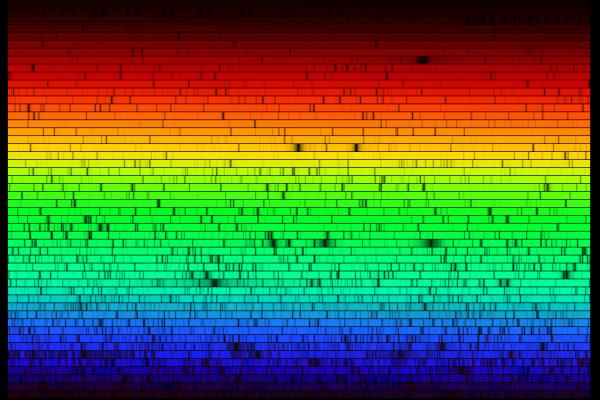
\includegraphics[width=\textwidth]{solarspectrum.jpg}\EC
}

\frame{\frametitle{\textbf{Announcements}}
\Large
\BI
\item Exam 3 on Tuesday
\pause
\item Study guide and last year's exam posted
\item Solutions to last year's exam will be posted on Friday
\item Extra study sessions for groups of 4+ only: Friday 2-5, Saturday 10AM-1PM, in the Physics Clinic
\pause
\item Grade calculator posted on course website
\BI
\item Please don't email me about exactly how participation grades are calculated; I've not determined that yet
\EI
\EI

}

\frame{\frametitle{\bf Chemistry: all I want you to know}
\large
\BI
\item Electrons occupy certain {\bf energy levels}
\item The particular energies that these levels have is {\bf unique} to particular elements: hydrogen has different allowed energies than mercury or neon or sodium etc.
\item An atom can absorb a photon and jump up to a higher level, conserving energy
\item ... an atom in a higher level can emit photons, jumping back down, conserving energy.
\item The photon's energy is equal to the {\it difference} between the two energy levels
\EI

\BS
\BS
\BC ... that's it. :) 
\EC
}

\frame{


If I take hydrogen and tear the electrons off of the atoms with an electric current,
they'll ``fall'' back down, going through the energy levels down to $n=1$.

\BS

Sometimes they'll skip energy levels; sometimes they'll go in sequence.

\BS

If I do this to hydrogen, what color will we see?

\BS
\BS

\color{A}A: UV: we won't see it, since the transitions down to $n=1$ are in the UV\\

\BS

\color{B}B: Several shades of red: we'll see the transitions down to $n=2$, which are red\\ 

\BS

\color{C}C: Infrared: the transitions at the top are very low energy, corresponding to
infrared light which we can't see \\ 

\BS

\color{D}D: UV, IR, and red, all at once: all the transitions happen, but we only see the
red photons because of the limits of our eyes\\ 

\BS

\pause

\color{E}E: Orange, because this is Syracuse, darnit! 
}

\frame{
\Large
\BC
Complete {\it Lecture Tutorials} pp.63-69.

\BS
\BS
\normalsize
After this, we'll talk about another application of this idea.
\EC}


\frame{\frametitle{\bf Emission spectra}

\large

Every chemical element has a unique {\it spectrum}: the colors of light that it can emit and absorb.

\BS

Other colors simply pass through.

\BS

(Molecules have these spectra too: their electron energy levels are more complicated.)

}


\frame{\frametitle{\textbf{Emission and absorption spectra}}

\BC
\Large
(Demonstration on the document camera, as a reminder of last time)
\EC
}



\frame{

\BC
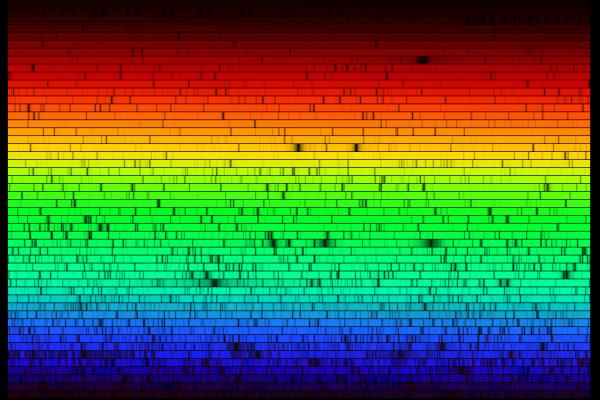
\includegraphics[width=0.7\textwidth]{solarspectrum.jpg}
\EC

\BI
\item The hot core of the Sun emits light of all wavelengths (thermal radiation)
\pause
\item The gases in the cooler atmosphere absorb light of their particular wavelengths
\pause
\EI
\BC
\color{Red} \large This picture tells us what's in the Sun!
\EC
}

\frame{

\Large

You discover lines in the solar spectrum that don't correspond to any known element.
What do you conclude?

\BS

\color{A}A: Something about quantum mechanics is different in the Sun\\\BS

\color{B}B: Something about light is different in the Sun\\\BS
\color{C}C: There's an element in the Sun that's not on Earth -- call it {\bf sunium} \\ \BS
\color{D}D: The extreme temperature of the Sun causes new lines to appear in its gas \\
}


\frame{

\BC
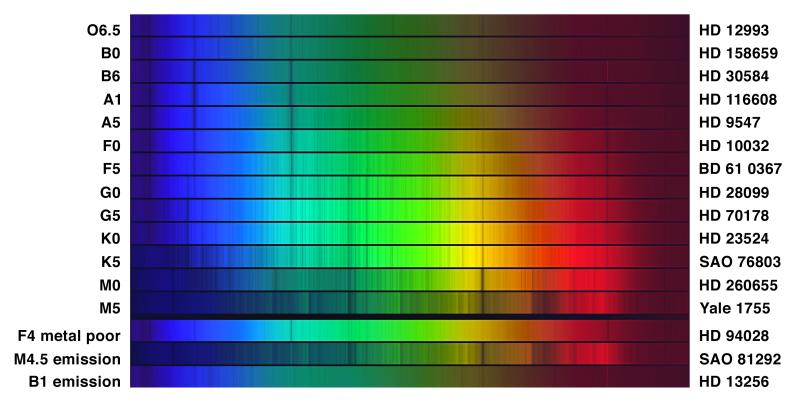
\includegraphics[width=0.95\textwidth]{stellar-spectra.jpg}
\BS

\large

All the stars are made of the same stuff -- the same stuff as we are.\pause
\EC
``The cosmos is also within us. We are made of star-stuff. We are a way for the universe to know itself.''

\begin{flushright}--Carl Sagan, {\it Cosmos} \end{flushright}
}

\frame{\frametitle{\textbf What a lucky accident!}
\large 
We're very lucky that atomic transitions happen to lie in our visual range!

There are others that are very interesting to astronomers:

\BI
\item Molecular vibrations: infrared
\pause
\item Molecular {\it rotations}: microwave
\pause
\item ``Hyperfine structure'' energy levels in hydrogen: 21 cm radio waves
\EI

\pause

\normalsize

This last is particularly interesting: it is a very particular frequency, echoing out from
all corners of the Universe, that says: hydrogen is here. (Hydrogen is 75\% of the universe.)
}

\frame{
\BC
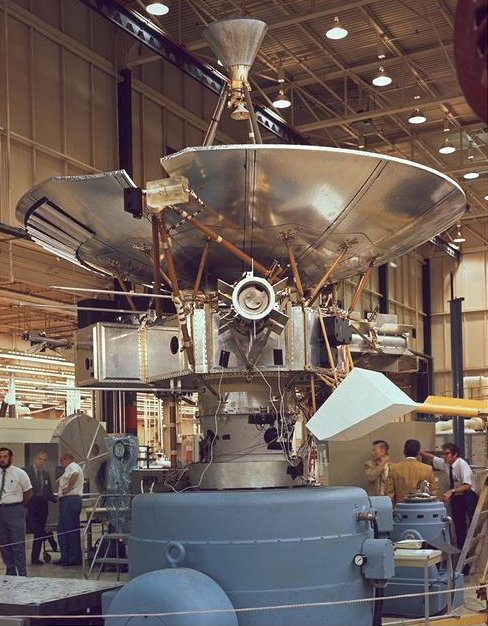
\includegraphics[width=0.5\textwidth]{pioneer-10.jpg}\\
\it
\small
The Pioneer 10 spacecraft (NASA)
\EC
}

\frame{
\BC
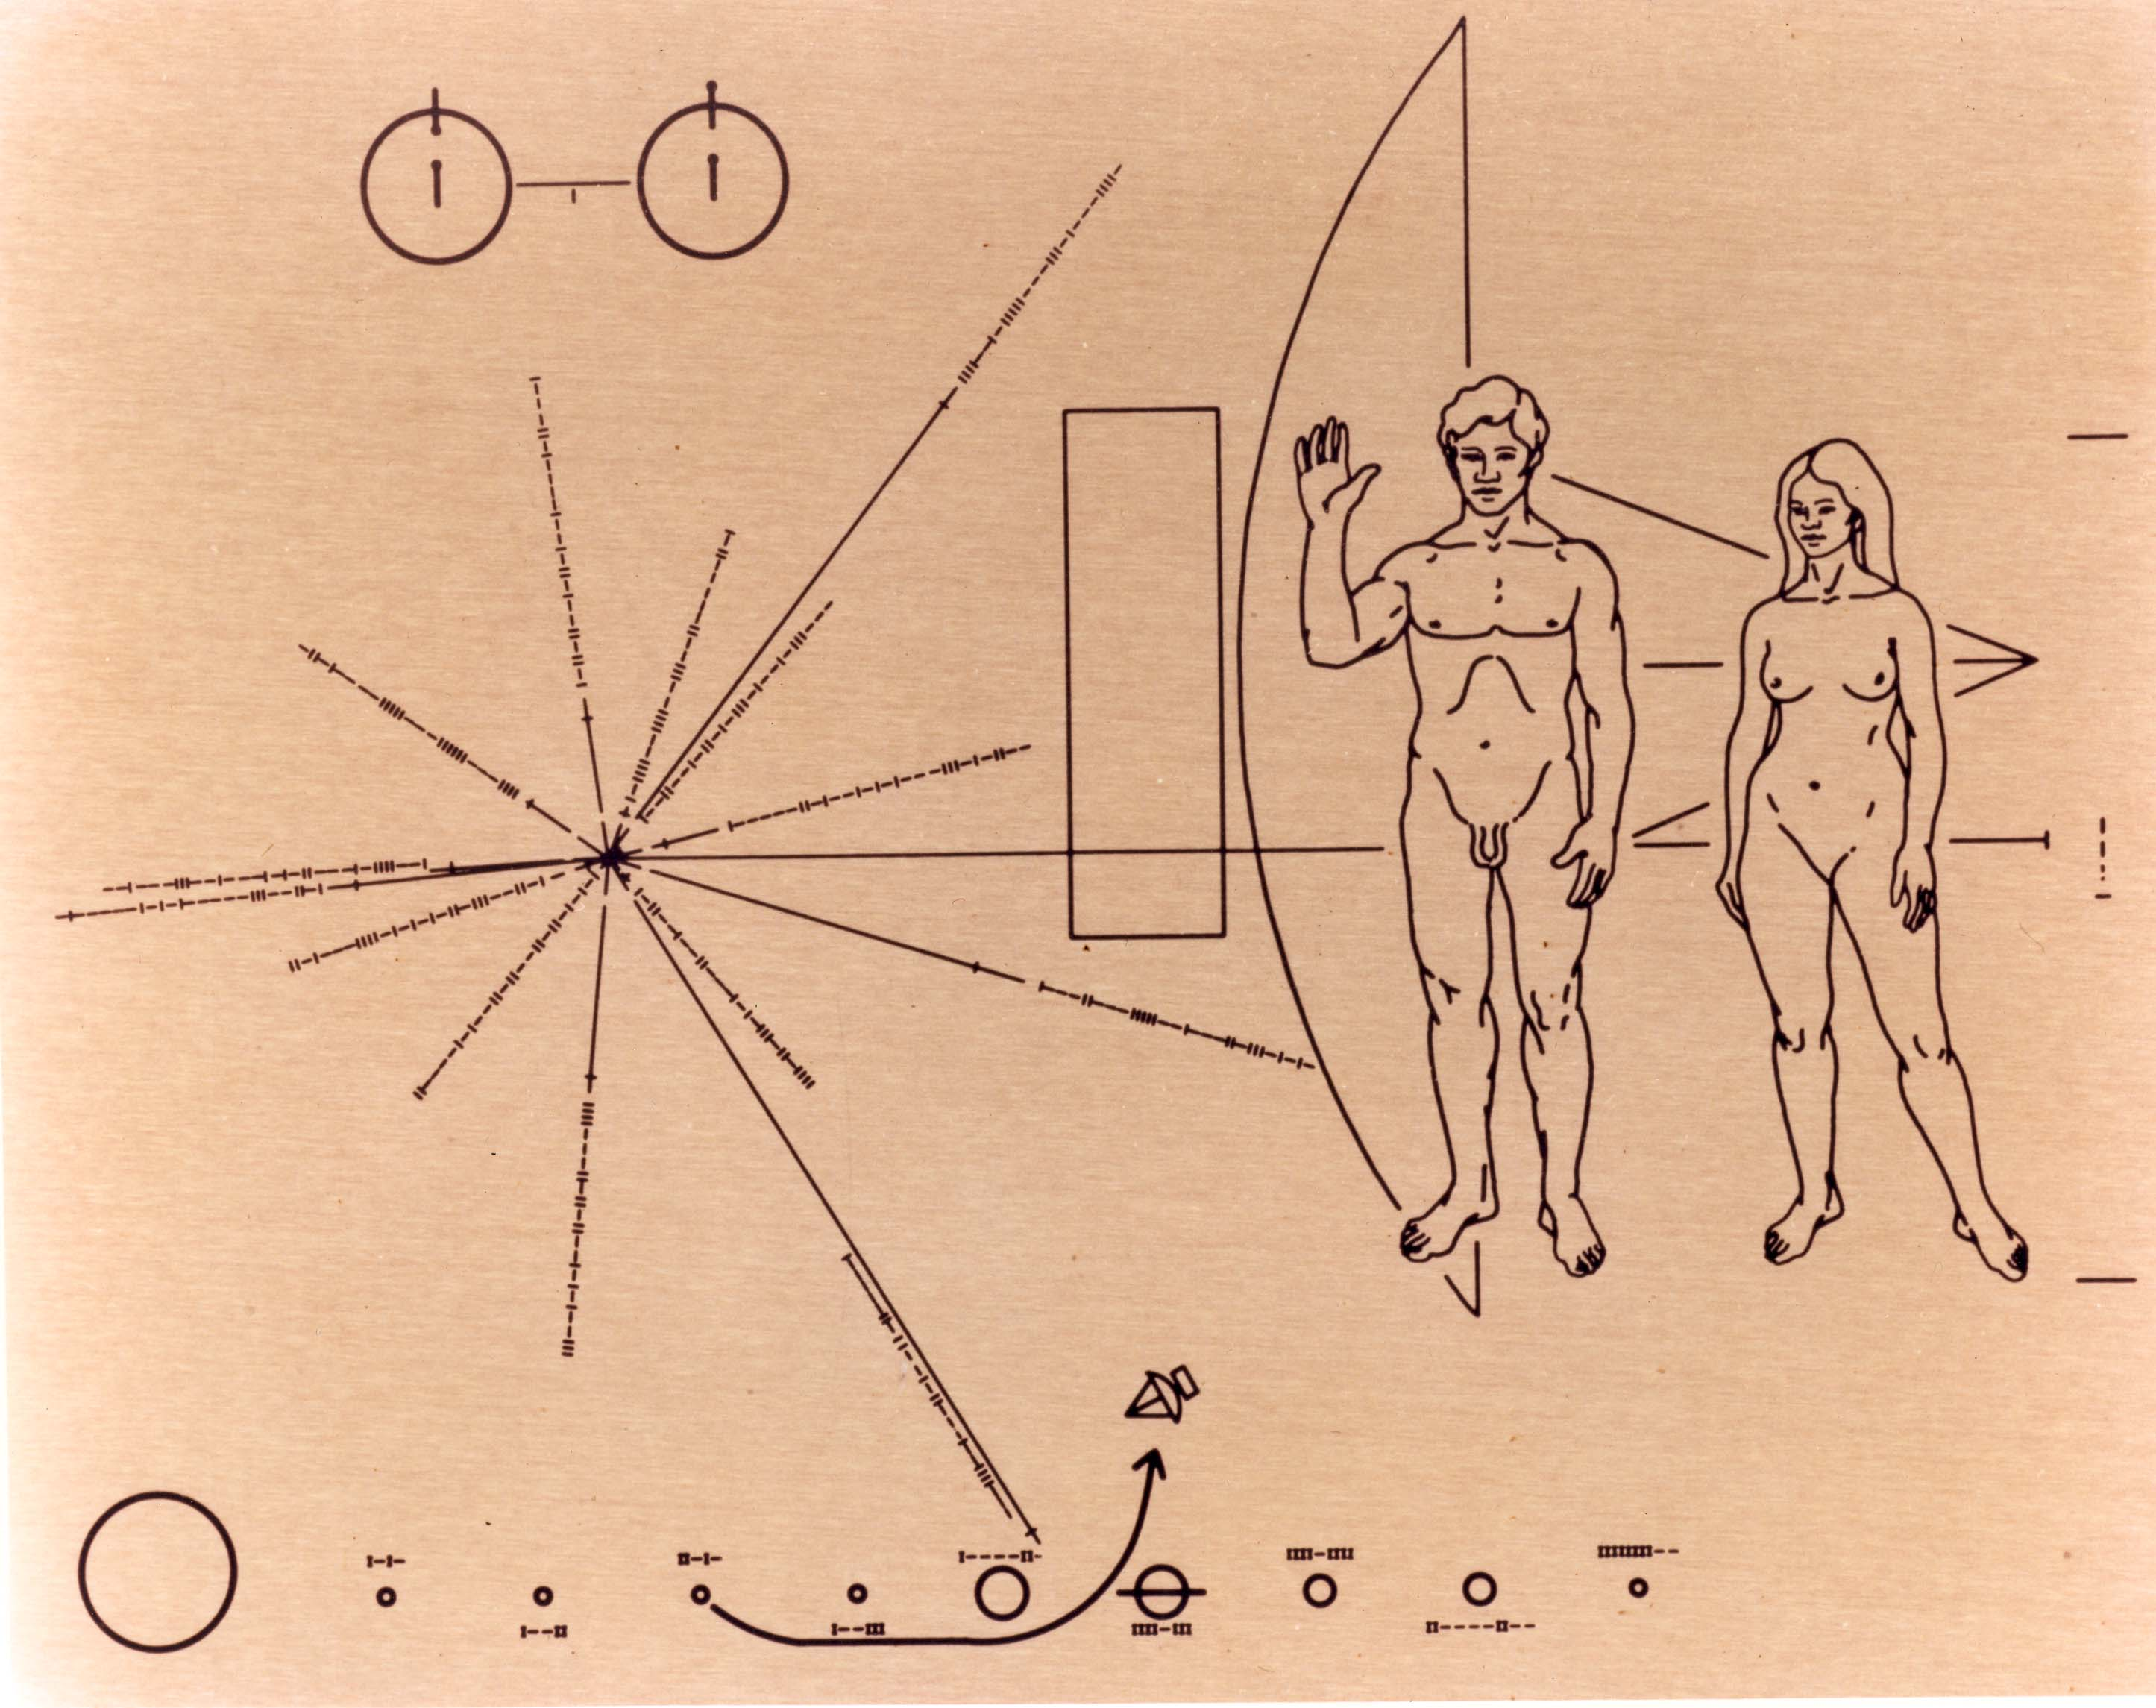
\includegraphics[width=0.8\textwidth]{pioneer-plaque.jpg}
\EC
}

\frame{
\BC
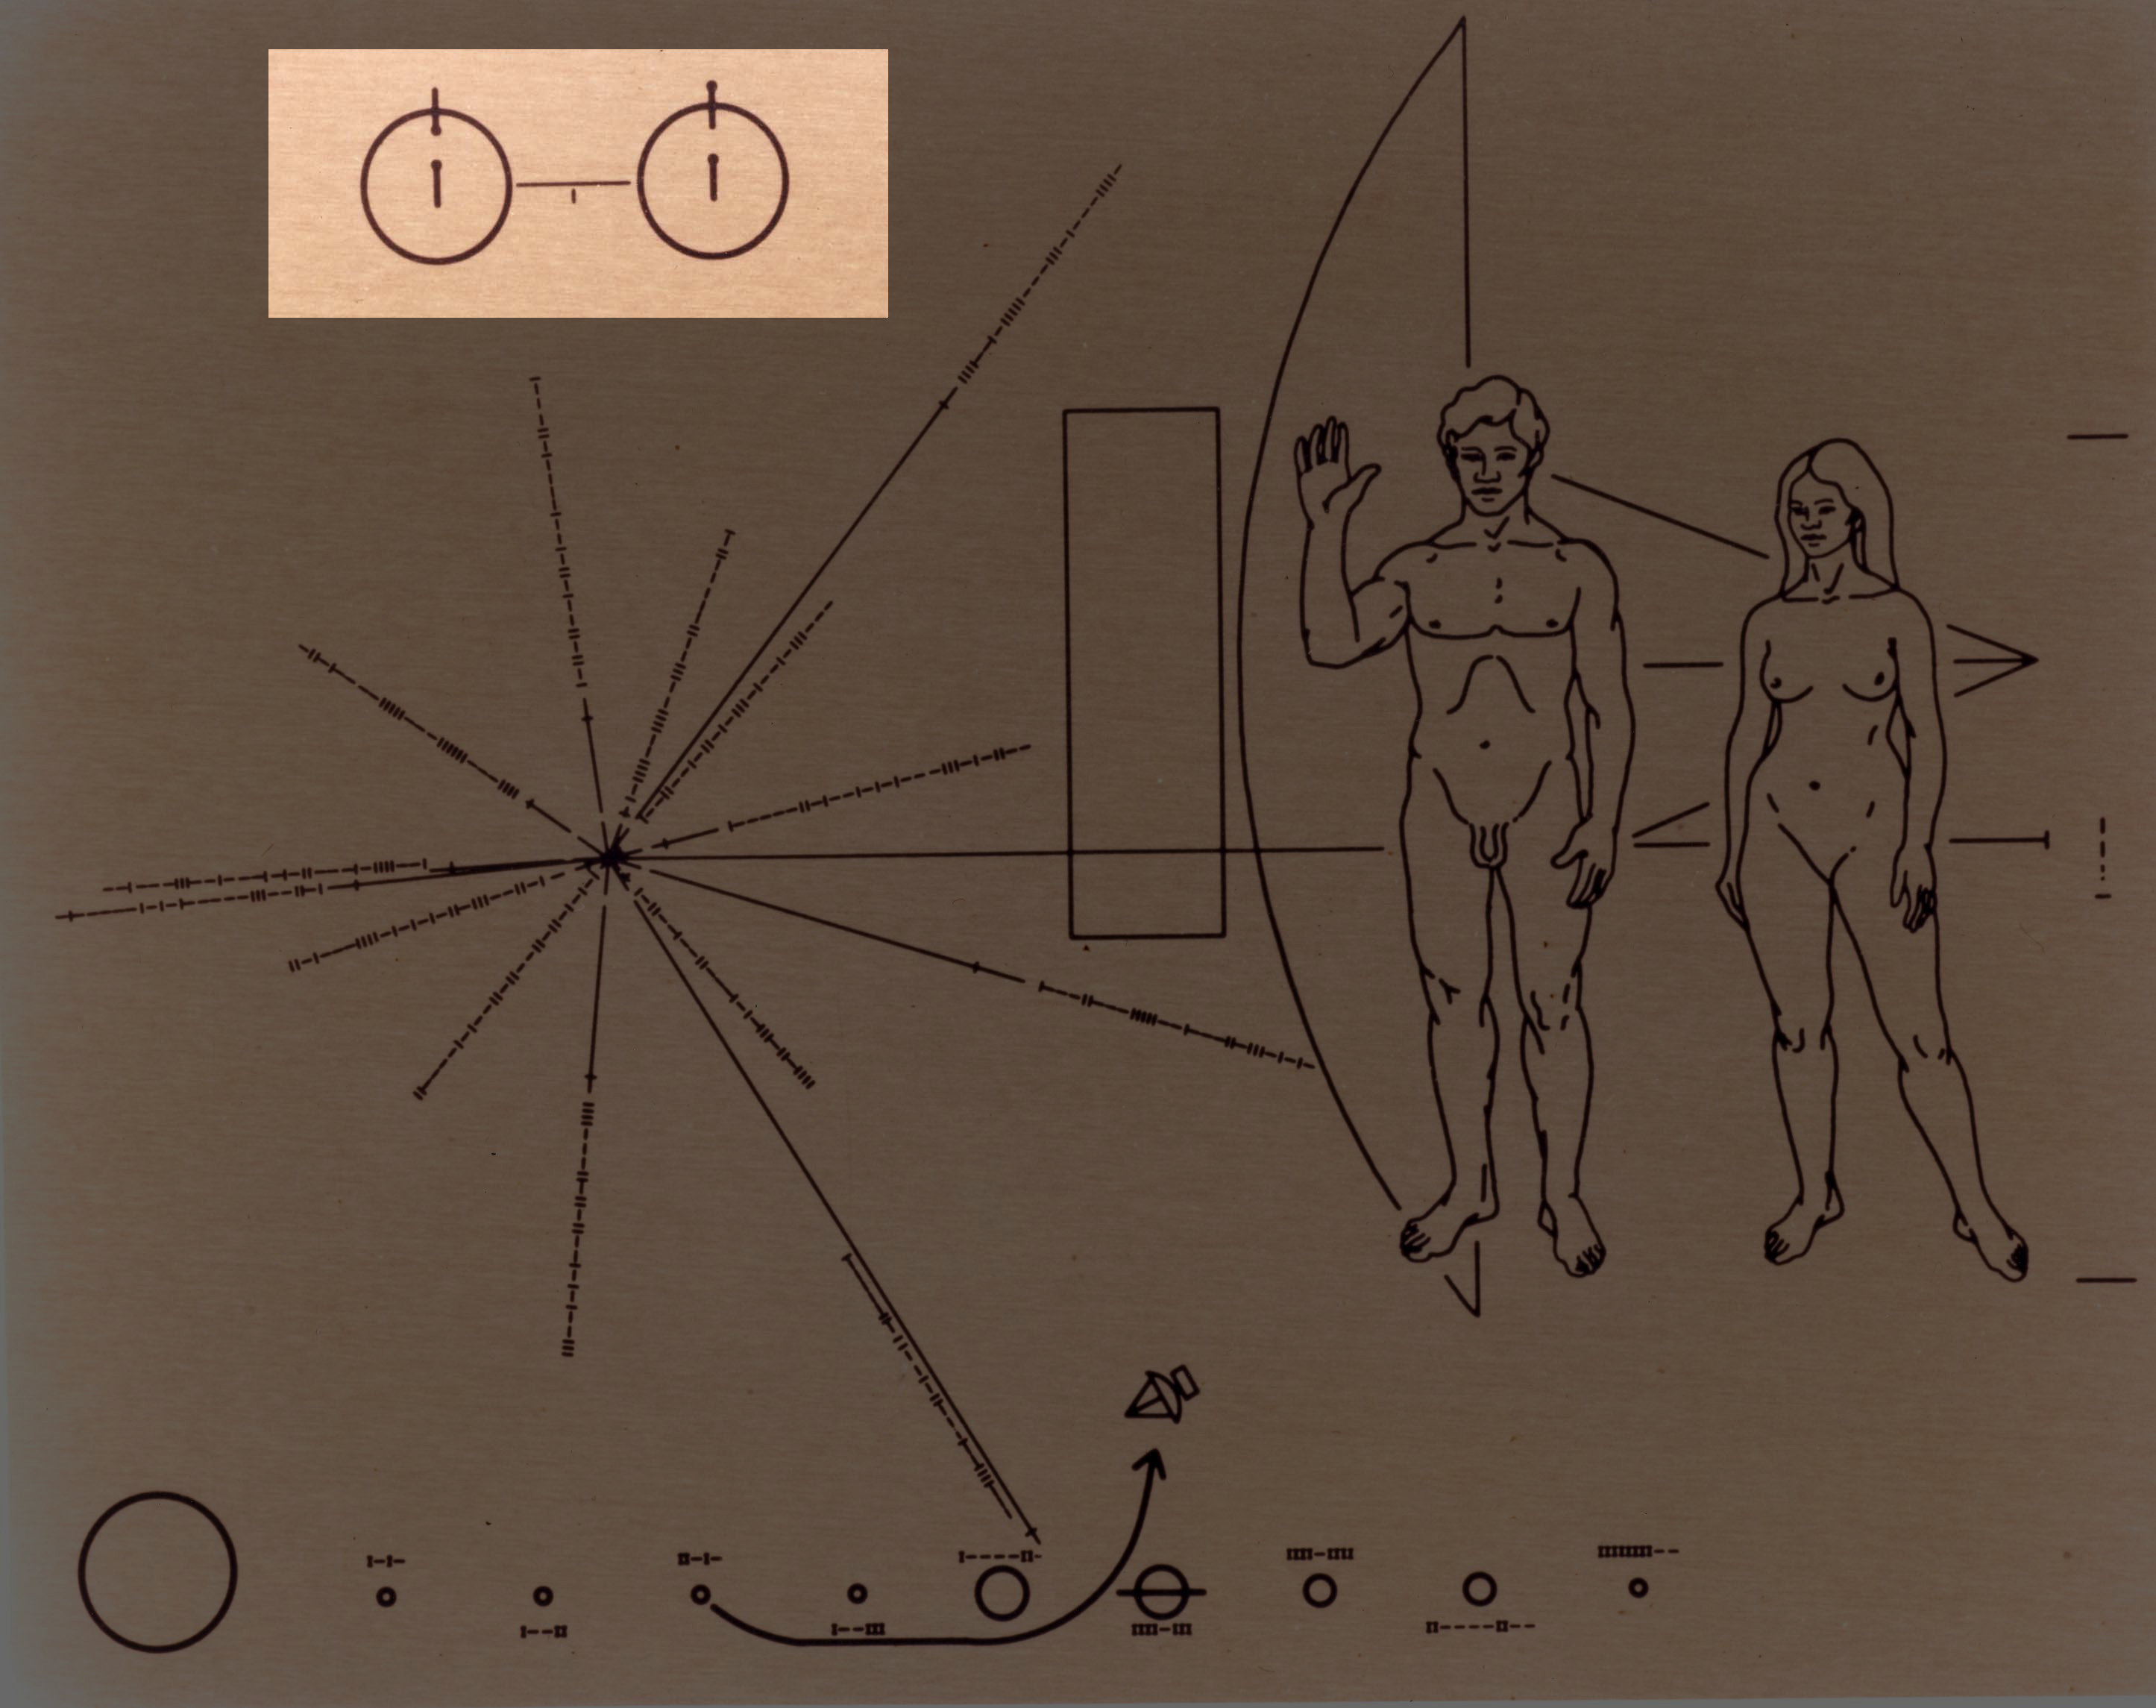
\includegraphics[width=0.7\textwidth]{pioneer-plaque-2.jpg}\\
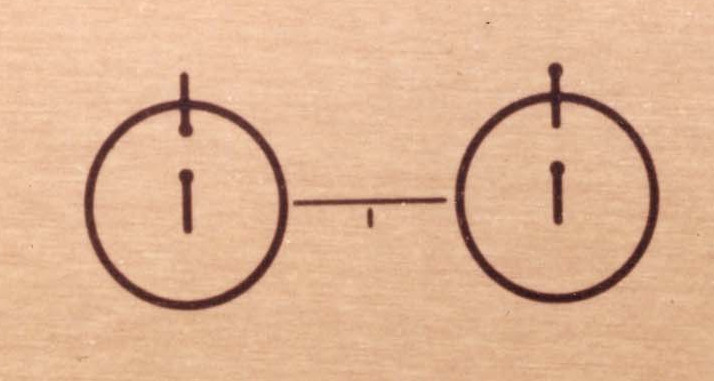
\includegraphics[width=0.3\textwidth]{hyperfine.jpg}
\EC
}

\frame{\frametitle{\textbf{The Sun's history and the source of its power}}

\BC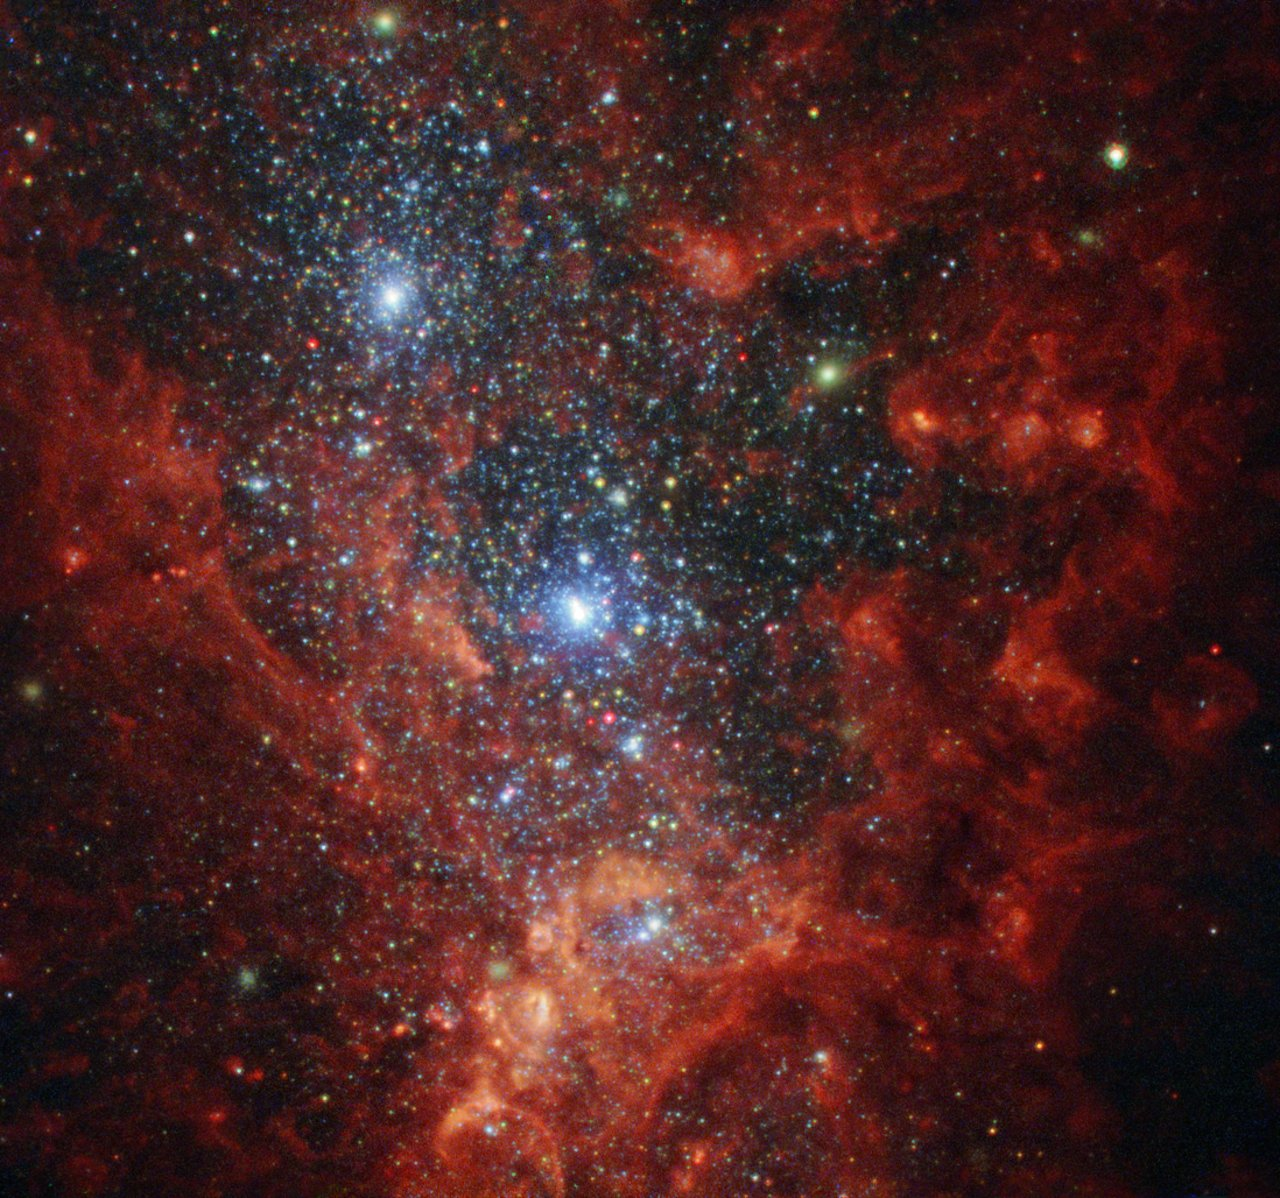
\includegraphics[width=0.5\textwidth]{hubble-formation.jpg}\\
\small (Hubble Space Telescope image: NASA + ESA / Judy Schmidt)

\BS

Clouds of gas -- mostly hydrogen but with a few heavier elements -- collapse
under their own gravity to form stars.

\EC
}

\frame{\frametitle{\textbf{The Sun's history and the source of its power}}
\Large
\BC
If you smash hydrogen nuclei together hard enough, they fuse to make helium
 -- plus two neutrinos -- plus a {\it lot} of energy.

\BS

$$(P) + (P) + (P) + (P) \rightarrow (NNPP) + 2e^+ + 2\nu$$

How much energy? Let's calculate it!

\pause\BS\BS

This {\color{Red} nuclear fusion} process converts hydrogen fuel into 
helium and a vast amount of energy. Could we harness it here on Earth?
\EC
}

\frame{\frametitle{\textbf{The Sun's fate and the fates of stars}}

\begin{columns}
\column{0.5\textwidth}
\normalsize

\BI
\item When the Sun runs out of hydrogen in its core, the core contracts,
while the outer layers puff up: it becomes a {\color{Red}red giant}. 
(5 billion years in the future, lasting for 1 billion years)

\item Eventually the core gets hot enough to fuse helium
into carbon, and the 
core ignites in a ``helium flash''. 

\item When the helium is depleted, that's it: the Sun isn't heavy enough
to fuse carbon

\item The carbon core will be left behind as a white dwarf, slowly cooling
-- a dying ember in the sky.

\item Its outer layers will be blown out into interstellar space,
briefly forming a nebula

\EI

\column{0.5\textwidth}

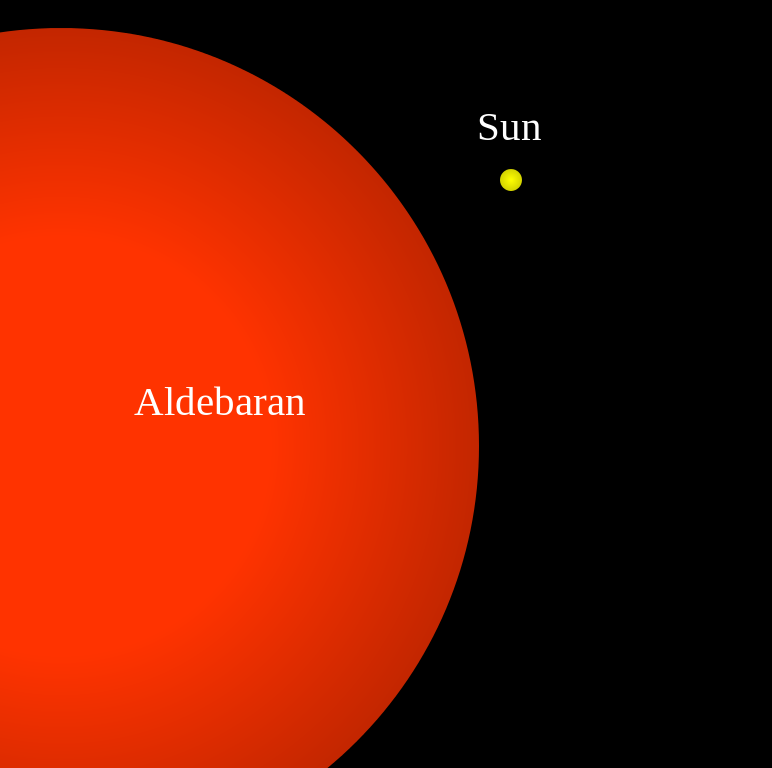
\includegraphics[width=0.9\textwidth]{aldebaran-sun.png}

\end{columns}
}






\end{document}

